\documentclass[12pt]{article}
\usepackage[utf8]{inputenc}
\usepackage{amsmath}
\usepackage{amsfonts}
\usepackage{amssymb}
\usepackage{hyperref}
\usepackage[a4paper, total={6in, 8in}]{geometry}
\usepackage{graphicx}
\usepackage{xcolor}
\usepackage{tcolorbox}
\usepackage{tikz}
\usepackage{array}
\usetikzlibrary{arrows,automata}
\usepackage{pgf}
\usepackage[ngerman]{babel} % Deutsche Sprache einstellen (neue Rechtschreibung)
\usepackage{listings}
\usepackage{xcolor}

\lstset{
    language=Python,
    basicstyle=\ttfamily\footnotesize,
    keywordstyle=\color{blue},
    stringstyle=\color{red},
    commentstyle=\color{green},
    showstringspaces=false,
    numbers=left,
    numberstyle=\tiny\color{gray},
    stepnumber=1,
    numbersep=10pt,
    breaklines=true,
    frame=single
}
\usepackage{xcolor}
\usepackage{tcolorbox}
\usepackage{tikz}
\usepackage{array}
\usetikzlibrary{arrows,automata}
\usepackage{pgf}
\usepackage[ngerman]{babel} % Deutsche Sprache einstellen (neue Rechtschreibung)


\definecolor{mytransparentcolor}{rgb}{0.8,0.2,0.3} % Beispiel RGB-Farbe


\definecolor{mytransparentcolor}{rgb}{0.8,0.2,0.3} % Beispiel RGB-Farbe

\title{N-Gramm Modell}
\author{
  Pötzsch Felix (580106)\\
  \and
  Borisov Timofei (580092) \\
  \and
  Furitsch Simon (578153)\\
}
\date{\today}

\begin{document}

% Title page
\maketitle

% Abstract
\begin{abstract}
	Dies ist ein Überblick zum Thema N-Gramme im Modul
	Aktuelle Themen der Informatik im Sommersemester 2024 an der
	Hochschule für Technik und Wirtschaft Berlin bei Prof. Dr. Tatiana Ermakova.
	Wir erklären Grundsätzlich was N-Gramme sind, wo sie eingeordnet werden können und wie mit dieser Technik umgegangen werden kann.
	Dazu zeigen wir einfache Optimierungen wie Smoothing, Back-Off Wording etc..
	Des weiteren werden wir ein Beispielprogramm aufführen anhand dessen wir nocheinmal
	die Verwendung von N-Grammen verdeutlichen.
\end{abstract}

% Table of contents
\tableofcontents
\clearpage

% Sections
\section{Einführung (Pötzsch, Felix)}

\subsection{Sprachmodelle}
Sprachmodelle sind der Versuch beispielsweise natürliche Sprache als mathematisches
Modell darstellen zu können. Ihnen liegt meist ein stochastischer Prozess zugrunde.
Bekannte Modelle sind:

\begin{itemize}
	\item RNN (Rekurrente Neuronale Netze)\cite[vgl.]{AIML2024}
	\begin{itemize}
        \item[-] Abhängigkeiten zwischen Wörtern können erfasst werden und so kontextuell, kohärente Sätze gebildet werden.
        \item[-] Verschwindender Gradient. Abhängigkeiten in großer Entfernung können nicht mehr erkannt werden.
    \end{itemize}
	\item LSTM (Long Short-Term Memory)\cite[vgl.]{AIML2024}
	\begin{itemize}
        \item[-] Art von RNN die das Problem des verschwindenden Gradienten durch Speicherzellen lösen.
        \item[-] Zelle ermöglicht selektives merken oder vergessen, wodurch langfristige Abhängigkeiten berücksichtigt werden können.
    \end{itemize}
	\item GRU (Gated recurrent Unit)\cite[vgl.]{AIML2024}
	\begin{itemize}
        \item[-] Zielen darauf ab, die Architektur von LSTMs zu vereinfachen und gleichzeitig das Problem des verschwindenden Gradienten anzugehen.
        \item[-] Weniger Gating- Mechanismen aber dafür Rechenintensiver.
        \item[-] Haben eine vergleichbare Leistung wie LSTM.
    \end{itemize}
	\item Transformer Modelle:\cite[vgl.]{AIML2024}
	\begin{itemize}
		\item[-] GPT (Generative Pre-Trained Transformer)
		\begin{itemize}
			\item[-] Im Gegensatz zu RNN benutzen Transformer Selbstaufmerksamkeitsmechanismen.
			\item[-] Transformatoren verarbeiten Wörter parallel, was zu höherer Effizienz führt.
		\end{itemize}
        \item[-] GPT4 (Generative Pre-Trained Transformer 4)
		\begin{itemize}
			\item[-] Ist im Gegensatz zu GPT3 (1,76 Billionen Parameter) kein monolithisches Sprachmodell mehr sondern eher eine Mischung aus 8 x 220 Milliarden Parametermodellen. \cite{Spriesterbach2023}
			\item[-] Umfangreicher Textkorpus.
			\item[-] Besonders gut für kohärente und kontextrelevante Texte.
			\item[-] Kann für Vielzahl von Anwendungen verwendet werden, z.B.: Code-generierung.
		\end{itemize}
    \end{itemize}
\end{itemize}


Im Voraus sollten bei diesen Modellen sowohl Kenntnisse über Sprache im Allgemeinen bestehen, sowie über die jeweilige Kommunikationssituation. Die oben genannten Modelle bestehen zudem aus mehreren Teilmodellen. Meist sind das Vokabular, Häufigkeiten und Grammatik. Die oben genannten Modelle treten zudem in Kombination auf.
Sprachmodelle lassen sich in 4 verschiedene Sorten einteilen:

\begin{itemize}
	\item Regelbasierte Systeme \cite[vgl.]{thamm}
	\begin{itemize}
		\item[-] Vordefinierte Sprachregeln, Vorlagen.
		\item[-] Fehlende Fähigkeit kontextrelevante dynamische Text zu generieren.
	\end{itemize}
	\item Vorlagenbasierte Systeme
	\begin{itemize}
		\item[-] Vordefinierte Vorlagen, die mit dynamischen Inhalten gefüllt werden.
		\item[-] Gewisses Maß an Anpassung möglich (Grammatik).
		\item[-] Kein einzigartiger kreativer Text.
	\end{itemize}
	\item Statistische Sprachmodelle
	\begin{itemize}
		\item[-] N-Gramme, Markov (HMM)
		\item[-] Mangel an semantischem Verständnis und Schwierigkeiten kontextrelevante Inhalte zu erzeugen.
	\end{itemize}
	\item Neuronale Sprachmodelle
	\begin{itemize}
		\item[-] Dialoge sind möglich und es können sowohl Kontextrelevante als auch Kohärente Teile erkannt werden.
		\item[-] Siehe RNN, LSTM, GRU, GPT
	\end{itemize}
\end{itemize}

\subsection{N-Gramme}
N-Gramme, sind in der Linguistik eine Sequenz von N aufeinanderfolgenden Fragmenten eines Textes.
Fragmente können dabei Buchstaben, Silben, Laute oder Wörter sein. Das können von 1-Gramm (Uni-Gramme),
über 2-Gramm (Bi-Gramme), 3-Gramm (Tri-Gramme) bis Multigrammen sein. Ihnen zugrunde liegt die Markov-Annahme.
Die Markov-Annahme\cite{scheffervanck2019} erschließt eine Vorhersage über einen zukünftigen Zustand nicht aus der Menge aller
Zustände, sondern nur der unmittelbaren vorherigen eingetretenen Zustände. Die Zustände können in diesem
Falle als Fragmente aufgefasst werden. Die klassischen Anwendungsgebiete für N-Gramme liegen in der
Rechtschreibkorrektur, Textvervollständigung/Wörter vorhersage (z.B.: SMS schreiben), Textanalyse
(Beurteilung), Spracherkennung (Audioanwendungen) und Handschrifterkennung.\\

\noindent Typische N-Gramme:

Unigramm:
$N = 1$: 	\fbox{\raisebox{0pt}[0.3cm][0.05cm]{\strut This}}
			\fbox{\raisebox{0pt}[0.4cm][0.15cm]{\strut is}}
			\fbox{\raisebox{0pt}[0.5cm][0.25cm]{\strut a}}
			\fbox{\raisebox{0pt}[0.6cm][0.35cm]{\strut sentence}}.
			\begin{tikzpicture}[baseline={(current bounding box.center)}]
				\coordinate (A) at (0,0.4);
				\coordinate (B) at (3,1);
				\coordinate (C) at (0,-0.2);
				\coordinate (D) at (3,-1);
				\draw (A) -- (B);
				\draw (C) -- (D);
			\end{tikzpicture}
			\begin{tikzpicture}[baseline={(current bounding box.center)}]
				\node at (2,0.9) {This};
				\node at (2,0.3) {is};
				\node at (2,-0.3) {a};
				\node at (2,-0.9) {sentence};
			\end{tikzpicture}\\[0.5cm]

Bigramm:
$N = 2$: 	\fbox{\raisebox{0pt}[0.3cm][0.05cm]{\strut This is}}
			\hspace{-0.6cm}\fbox{\hspace{0.4cm}\raisebox{0pt}[0.4cm][0.15cm]{\strut a}}
			\hspace{-0.6cm}\fbox{\hspace{0.4cm}\raisebox{0pt}[0.5cm][0.25cm]{\strut sentence}}.
			\begin{tikzpicture}[baseline={(current bounding box.center)}]
				\coordinate (A) at (0,0.4);
				\coordinate (B) at (3,1);
				\coordinate (C) at (0,-0.2);
				\coordinate (D) at (3,-1);
				\draw (A) -- (B);
				\draw (C) -- (D);
			\end{tikzpicture}
			\begin{tikzpicture}[baseline={(current bounding box.center)}]
				\node at (2,0.9) {This is};
				\node at (2,0.3) {is a};
				\node at (2,-0.3) {a sentence};
			\end{tikzpicture}\\[0.5cm]

Trigramm:
$N = 3$: 	\fbox{\raisebox{0pt}[0.3cm][0.05cm]{\strut This is a}}
			\hspace{-0.6cm}\fbox{\hspace{0.4cm}\raisebox{0pt}[0.4cm][0.15cm]{\strut sentence}}.
			\begin{tikzpicture}[baseline={(current bounding box.center)}]
				\coordinate (A) at (0,0.4);
				\coordinate (B) at (3,1);
				\coordinate (C) at (0,-0.2);
				\coordinate (D) at (3,-1);
				\draw (A) -- (B);
				\draw (C) -- (D);
			\end{tikzpicture}
			\begin{tikzpicture}[baseline={(current bounding box.center)}]
				\node at (2,0.9) {This is a};
				\node at (2,0.3) {is a sentence};
			\end{tikzpicture}\\[1cm]


\noindent Die daraus folgende typische Markov Annahme als Prozessdiagramm und Übergangstabelle würde dazu folgend aussehen:\\

\begin{minipage}{0.50\textwidth}
	\begin{tikzpicture}[->,>=stealth',shorten >=1pt,auto,node distance=2.8cm, semithick]

		\tikzstyle{every state}=[fill=white,draw=black,text=black]

		\node[initial,state] (A)                    {$Z_1$};
		\node[state]         (B) [below right of=A] {$Z_2$};
		\node[state]         (C) [above right of=B] {$Z_3$};

		\path 	(A) edge [loop above] node {0.3} (A)
				(B) edge node {0.3} (A)
				(A) edge node {0.7} (B)
				(B) edge [loop below] node {0.3}
				(B)	edge              node {0.4} (C)
				(C) edge [loop above] node {1} (C);

	\end{tikzpicture}
\end{minipage}
\begin{minipage}{0.45\textwidth}
	\begin{tabular}{ m{1cm} | m{1cm}| m{1cm} | m{1cm} }
		& $Z_1$ & $Z_2$ & $Z_3$\\
		\hline
		$Z_1$ & 0.3 & 0.3 & 0\\
		\hline
		$Z_2$ & 0.7 & 0.3 & 0\\
		\hline
		$Z_3$ & 0 & 0.4 & 1\\
		\hline
		$=$ & 1 & 1 & 1\\
	\end{tabular}
\end{minipage}\\[1cm]

\noindent Grundsätzlich haben wir es mit bedingten Wahrscheinlichkeiten zu tun die wie folgt lauten:\\

\begin{equation}
	\begin{split}
	P(t) = P(w_1, w_2,...w_n) &= P(w_1)*P(w_2 \mid w_1)...P(w_n \mid w_1,...w_n-1) \\
	&= \prod_{i=1}^{n} P(w_i \mid w_1...w_i-1)
	\end{split}
\end{equation}

\begin{equation}
	P(w_1 \mid w_1...w_i-1) = \frac {P(w_1...w_i)}{P(w_1...w_i-1)}
\end{equation}
\\
Also die Wahrscheinlichkeit, dass Wort 1 eintritt unter der Bedingung, dass ein Paar andere Wörter vorher
schon in Kombination aufgetreten sind. Demnach wird Text auf Basis von statistischen Mustern generiert
oder anders gesagt: Neu angeordnet. Es mangelt dadurch häufig an semantischem Verständnis. Insbesondere
im Zusammenhang mit langfristigeren Abhängigkeiten (Kohärenz) sind Sprachmodelle die rein auf N-Grammen
basieren sehr ungeeignet, um Texte zu schreiben. Da lediglich auf Basis einer \textit{Maximum-Likelyhood}\cite{scheffervanck2019} Methode
gearbeitet wird, kann Text nur \textit{nacherzählt} werden aber nicht generiert.\\
Es folgen nun ein paar typischen Eigenheiten von N-Grammen. Einem Totalversagen entgegenzuwirken, muss
zunächst die Wahl eines geeigneten N priorisiert werden. Denn auch wenn ein geeigneter (Text-) Korpus
gut gewählt wurde kann es zu \textit{Unseen N-Grams}\cite{markert2019} kommen. Ebenso wie \textit{Unseen N-Grams}\cite{markert2019} gibt es
auch \textit{Unseen/Unknown Words}\cite{markert2019}. Prinzipiell aber sollte gesagt werden, dass auch ein großer oder geeigneter Korpus nicht immer zum
Erfolg führt, da auch dort Wortkombinationen oder Wörter \textit{Unseen} sein können (Chomsky, Zipfsches Gesetz).\cite{markert2019}
Des Weiteren sollte auf den Underflow bei der Bewertung der Wahrscheinlichkeiten geachtet werden. Dieses
Problem führt zum nächsten, denn es müssen nicht nur zu niedrige, sondern auch die vollständigen
Nullwahrscheinlichkeiten beachtet werden.\\
Es müssen also vor allem die Informationen in Form der Angepasstheit sowie Auswahl vorab gut gewählt werden
sowie die im Folgenden beschrieben Techniken des \textit{Smoothings}\cite{markert2019}, also der Re-evaluation von
Nullwahrscheinlichkeiten und niedrigen Wahrscheinlichkeiten eigesetzt werden. Dazu zählt ebenfalls die
zusätzlich im Folgenden beschriebene Perplexität als Evaluationstechnik, um auf \textit{Back Off Words}\cite{markert2019}, also
Wörter, auf welche ausgewichen werden kann, zu kommen.


\section{Fortgeschrittene Konzepte und Techniken in N-Gramm-Modellen (Borisov, Timofei)}
\subsection{Was ist un-seen N-Grams?}
Da jeder Corpus begrenzt ist, fehlen darin zwangsläufig einige völlig akzeptable Wortfolgen. Das heißt, wir werden viele Fälle von vermeintlichen "Zero Probability n-grams" haben, die in Wirklichkeit eine Nicht-Null-Wahrscheinlichkeit haben sollten \cite{jurafsky2023}.

Betrachten wir die Wörter, die auf das Bigram aus Daniel Jurafskys Buch basieren. Ein Textkorpus zusammen mit ihrer Anzahl:

\begin{itemize}
	\item denied the allegations: 5
	\item denied the speculation: 2
	\item denied the rumors: 1
	\item denied the report: 1
\end{itemize}

Aber nehmen wir an, unser Testsatz enthält Sätze wie:
\begin{itemize}
	\item denied the offer
	\item denied the loan
\end{itemize}

P(offer|denied the) ist 0!
P(loan|denied the) ist 0!

Diese Nullen bedeuten, dass wir die Wahrscheinlichkeit anderer Wortkombinationen stark unterschätzt haben, was die richtige Entscheidung der Anwendung, die auf unserem Modell läuft, stark beeinflussen könnte.

Das Problem heißt “Data Sparsity”\cite{dremio2023}. Also kurz gesagt, das bedeutet, dass viele Daten in einem Datensatz fehlen oder auf Null gesetzt sind, sodass die meisten Zellen in einer Tabelle leer bleiben. Dies tritt häufig bei spärlichen Matrizen oder hochdimensionalen Datensätzen auf, wo nicht alle Elemente beobachtet oder erfasst werden. Was können wir also mit den Wörtern machen, die wir verwenden und die nicht in den Kontext unserer Trainingsdaten passen?

Die Methode zur Lösung dieses Problems heißt: Smoothing oder Discounting.

\subsection{Smoothing Techniques}
\subsubsection{Laplace-Glättung. Add One (Add X).}
Die einfachste Art der Glättung besteht darin, zu allen n-Gramm-Zählungen einen Wert zu addieren, bevor wir sie zu Wahrscheinlichkeiten normalisieren. Alle Zählungen, die vorher Null waren, haben nun den Wert 1, die Zählungen von 1 werden zu 2 usw. Dieser Algorithmus wird als Laplace-Glättung oder Additive Glätterung bezeichnet \cite{foster2020}.

Statt
\begin{center}
	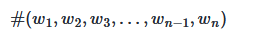
\includegraphics[width=0.3\textwidth]{statics/Borisov/1.PNG}
\end{center}

Wir setzen
\begin{center}
	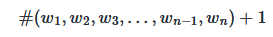
\includegraphics[width=0.4\textwidth]{statics/Borisov/2.PNG}
\end{center}

Da das Vokabular aus V-Wörtern besteht und jedes Wort inkrementiert wurde, müssen wir auch den Nenner anpassen, um die zusätzlichen V-Beschachtungen zu berücksichtigen.
\begin{center}
	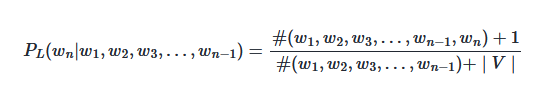
\includegraphics[width=0.6\textwidth]{statics/Borisov/3.PNG}
\end{center}

\cite{maucher2022}

Eine Alternative zur Glättung durch Addition besteht darin, einen etwas geringeren Anteil der Wahrscheinlichkeitsmasse von den gesehenen zu den ungesehenen Ereignissen zu verschieben. Anstatt zu jeder Zählung 1 zu addieren, fügen wir einen Bruchteil der Zählung k hinzu.
\begin{center}
	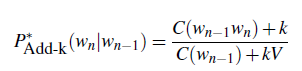
\includegraphics[width=0.4\textwidth]{statics/Borisov/4.PNG}
\end{center}

\cite{jurafsky2023}.

\subsubsection{Good-Turing Glättung}
Wie berechne ich die Wahrscheinlichkeit von un-seen N-Grams?

Der erste Schritt der Berechnung besteht darin, die Wahrscheinlichkeit abzuschätzen, dass ein zukünftig beobachtetes Fall zu einer bisher nicht gesehenen Art gehört. Diese Schätzung ist:
\begin{center}
	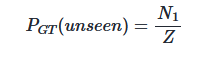
\includegraphics[width=0.3\textwidth]{statics/Borisov/5.PNG}
\end{center}

Der nächste Schritt besteht darin, die Wahrscheinlichkeit zu schätzen, dass das nächste beobachtete Fall einer Art angehört, die bereits r-mal beobachtet wurde. Für eine einzelne Art beträgt diese Schätzung:
\begin{center}
	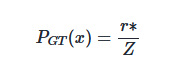
\includegraphics[width=0.2\textwidth]{statics/Borisov/6.PNG}
\end{center}
Good-Turing-Smoothing löst dieses Dilemma, indem es die Häufigkeitswerte anpasst. Es wird so getan, als ob Arten, die eigentlich r-mal vorkommen, \( r^* \)-mal vorkommen, mit
\begin{center}
	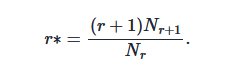
\includegraphics[width=0.3\textwidth]{statics/Borisov/7.PNG}
\end{center}
\cite{maucher2022},\cite{gale1995}

\subsubsection{Katz Backoff Glättung}
\quad Wenn ein benötigtes n-Gramm in einem Backoff-N-Gramm-Modell keine Vorkommen aufweist, gehen wir zum (n-1)-Gramm über. Dieser Prozess wird fortgesetzt, bis wir eine Sequenz finden, die einige Vorkommen hat.
\\ Damit ein Backoff-Modell eine korrekte Wahrscheinlichkeitsverteilung ergibt, müssen die n-Gramme höherer Ordnung reduziert werden, um etwas Wahrscheinlichkeitsmasse für die n-Gramme niedrigerer Ordnung zu reservieren. Ähnlich wie bei der Add-One-Glättung führt die Verwendung der nicht diskontierten MLE-Wahrscheinlichkeit dazu, dass bei der Ersetzung eines n-Gramms mit einer Wahrscheinlichkeit von Null durch ein n-Gramm niedrigerer Ordnung zusätzliche Wahrscheinlichkeitsmasse hinzugefügt wird. Dies würde dazu führen, dass die Gesamtwahrscheinlichkeit, die das Sprachmodell allen möglichen Zeichenketten zuweist, größer als 1 ist. Neben diesem expliziten Abzinsungsfaktor benötigen wir eine Funktion a, um diese Wahrscheinlichkeitsmasse auf die n-Gramme niedrigerer Ordnung zu verteilen.
\\ \\Beim Katz-Backoff stützen wir uns auf eine diskontierte Wahrscheinlichkeit P*, wobei wir rekursiv auf die Katz-Wahrscheinlichkeit für das (n-1)-Gramm mit kürzerer Vorgeschichte zurückgehen. Die Wahrscheinlichkeit für ein Backoff n-Gramm PBO wird also wie folgt berechnet:
\begin{center}
	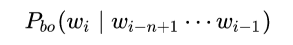
\includegraphics[width=0.4\textwidth]{statics/Borisov/8.PNG}
\end{center}
\begin{center}
	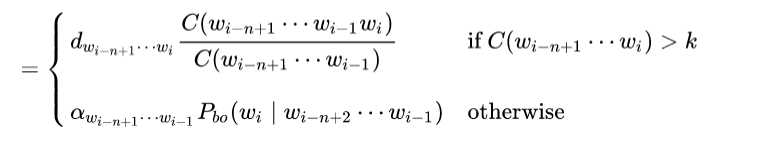
\includegraphics[width=0.7\textwidth]{statics/Borisov/9.PNG}
\end{center}

\quad Zur Berechnung von $\alpha$ ist es sinnvoll, zunächst eine Größe $\beta$ zu definieren, die die verbleibende Wahrscheinlichkeitsmasse für das $(n - 1)$-Gramm darstellt:


\begin{center}
	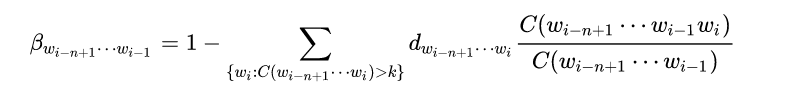
\includegraphics[width=0.8\textwidth]{statics/Borisov/10.PNG}
\end{center}

Anschließend:

\begin{center}
	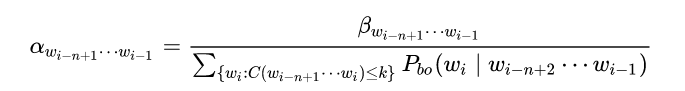
\includegraphics[width=0.8\textwidth]{statics/Borisov/11.PNG}
\end{center}

\subsection{Vergleich von N-Grammen und neuronalen Netzen.}
\quad Im Allgemeinen sind neuronale Netze fortschrittlichere und komplexere Instrumente als N-Gramme. Ihr Vorteil liegt in vielen Aspekten. Zum Bespie: N-Gramme erfassen nur den lokalen Kontext. Ein Trigramm-Modell berücksichtigt nur zwei vorangehende Wörter, um das nächste Wort vorherzusagen. Sie sind nicht in der Lage, weitreichende Abhängigkeiten zu verstehen. Mit steigendem Wert von "n" wächst die Zahl der möglichen n-Gramme exponentiell, was zu hohem Speicherverbrauch und Sparsamkeitsproblemen führt. Probleme mit Wörtern, die mehrere Bedeutungen haben (Polysemie), oder mit verschiedenen Wörtern, die gleich klingen (Homonymie), weil ihnen ein tiefes Verständnis des Kontextes fehlt. N-Grams erfordern manuelles Feature-Engineering, um die relevanten n-Gramme auszuwählen, und führen oft zu hochdimensionalen, spärlichen Vektoren usw. \cite{roshmita2023} \cite{clarkGiorgoloLappin}
\\
\quad Neuronale Netze sind mittlerweile kontextbewusst. Insbesondere mit Architekturen wie LSTM (Long Short-Term Memory) oder Transformer-Modellen können neuronale Netze weitreichende Abhängigkeiten und kontextuelle Informationen über ganze Sätze oder sogar Absätze hinweg erfassen. Sie verfügen über ein automatisches Lernen von Merkmalen während des Trainingsprozesses, wodurch sich der Bedarf an umfangreicher manueller Merkmalstechnik verringert usw.Wir müssen jedoch den Vorteil von N-Grammen anerkennen. Bei kurzen Texten sind N-Gramm-Methoden dem neuronalen Netz überlegen.
\cite{babukumar2010}

\section{Konkrete Schritte zur Implementierung eines N-Gramm Modells in Pyhton (Furitsch, Simon)}
\subsection{Datenvorbereitung}
\quad Die Daten müssen zuerst in ein für das Training geeignetes Format gebracht werden. Hierzu wird der Text zuerst in Kleinbuchstaben konvertiert und die Sonderzeichen und Zahlen werden entfernt. Textfehler, wie Beispielsweiße doppele Leerzeichen werden gemeinsam mir den \textbf{Stoppwörtern} bereinigt
\subsubsection{Stoppwörter}
\quad Stoppwörter sind Füllwörter, welche keine richtige Bedeutung für die Textvorhersage habe, ein Beispiel hierfür ist das Wort: „aber“
\subsubsection{Stemming und Lemming}
\quad Eine Möglichkeit das Modell anzupassen ist es die Wörter in eine andere Form zu bringen. Dies kann sich sowohl positiv als auch negativ auf das Modell auswirken, hierzu sei aber der Anwendungsfall von Bedeutung. Insbesondere ist hierbei auf das Evaluieren durch die in Kapitel 4.5 genannte \textbf{Perplexität} hingewießen. Diese kann dabei helfen die Auswirkung von Stemmung und Lemming zu ermitteln.
\\Beim \textbf{Stemming} wird das Wort einfach in seinen Wortstamm gesetzt: aus singen wird sing und aus gehen wird geh
\\Beim \textbf{Lemming} hingegen wird das Wort in seine Grundform gebracht. aus Häuser wird Haus und aus ging wird gehen
\subsection{Grundlagen}
\subsubsection{Bibliothek: NLTK}
\quad Im Kapitel 4.3 wird für den Code die Bibiothek NLTK verwendet. Natural Language Toolkit ist die populärste Bibliothek in der neurolighuistischen Programmierung. Diese Bibliothek macht unter anderem das Tokenisieren, die Erzeugung von Grams, das importieren verschiedener Textkörper und vieles weiteres zum Einzeiler. Auch in den folgenden Kapiteln werden die Funtionalitäten näher beleuchtet.
\subsubsection{Tokenisierung}
\quad Bei der Tokenisierung handelt es sich um die Aufteilung einer Zeichenkette in kleinere Teile. Die für n-Gram meist genutzte Tokenisierungsmethode ist die Tokenisierung in Wörtern da ja auch die Vorhersahe auf Wörtern basiert. Das bedeutet jedes Wort wird ein Token in der Lösungsmenge. Aus „Das ist ein Satz“, wird {„das“,“ist“,“ein“,“satz“}. Diese Menge wird dann verwendet, um die n-Grams zu erzeugen
\\In \textbf{NLTK} wird der Worttokenisierer mitgeliefert
\begin{lstlisting}
def tokenize(text):
    return nltk.word_tokenize(text.lower())
\end{lstlisting}
\subsubsection{Grams erzeugen}
\quad Nun werden die Tokens verwendet, um n-Gramme zu erzeugen. Die konkrete Zahl des n hängt stark von der Kontextanforderung an das Modell ab. Während niedrige n zum Beispiel Unigram (1-gram) und Biagram (2-gram) nützlich für Wortverbindungen und einen geringen Kontext sind, sind Modelle mit hohen n nützlich für die Schätzung von größeren Sätzen bzw. über einen längeren Kontext hinaus.
\\In \textbf{NLTK} ist dies wieder ganz einfach
\begin{lstlisting}
def getGram(gram, tokens):
    return list(nltk.ngrams(tokens, gram))
\end{lstlisting}
Dies ist eine Methode welche das n und die Tokens übergeben bekommt und daraus das gewünschte Gram erzeugt. Zum Beispiel n=2 alle Biagramme der Tokens. Für die Ermittlung der in Kapitel 4.2.4 genannten bedingten Wahrscheinlichkeiten ist es jedoch auch notwendig die Wahrscheinlichkeiten und somit auch die Grams der darunter liegenden Dimensionen zu ermitteln. Geht man also von n=3 aus sollten alle Unigramme, Biagramme und Triagramme erzeugt werden.
\begin{lstlisting}
def getGrams(n, tokens):
    grams = [[] for _ in range(n)]
    for i in range(1, n + 1):
        grams[i - 1] = getGram(i, tokens)
    return grams
\end{lstlisting}
\subsubsection{Bedingte Wahrscheinlichkeiten ermitteln}
\quad Die Wahrscheinlichkeiten werden nun ermittelt damit das Modell damit die Vorhersage bilden kann.
\\Dies passiert in zwei Schritten:
\begin{lstlisting}
def buildModel(grams):
    model = defaultdict(lambda: defaultdict(lambda: 0))
    for gram_list in grams:
        for gram in gram_list:
            prefix = gram[:-1]
            suffix = gram[-1]
            if prefix:  # Keine () -> Wort predictions
                model[prefix][suffix] += 1
    return model
\end{lstlisting}
Hier wird das Model einfach in einem zweidimensionalen Dictionary gespeichert. Der Schlüssel der ersten Dimension ist der Prefix, also alles bis auf das letzte Wort. Die zweite Dimension ist der Suffix, also das letze Wort. Der Wert dahinter ist die Anzahl wie oft der Suffix auf den Prefix gefolgt ist.
\begin{center}
	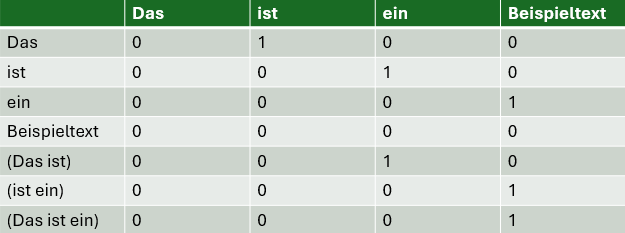
\includegraphics[width=0.8\textwidth]{statics/Furitsch/table.PNG}
\end{center}
\begin{lstlisting}
def convertToProbabilities(model):
    for prefix in model:
        total_count = sum(model[prefix].values())

        for suffix in model[prefix]:
            model[prefix][suffix] /= total_count
\end{lstlisting}
Hier wird nun ermittelt wie viel mögliche Suffixe es für einen Prefix gibt. Anschließend wird das Vorkommen der einzelnen Suffixe geteilt durch die Anzahl aller Suffixe denn das liefert uns die benötigten bedingten Wahrscheinlichkeiten.
\subsubsection{Vorhersage}
\begin{lstlisting}
def predict(model, prefix):
    if prefix in model:
        possible_words = model[prefix]
        return max(possible_words, key=possible_words.get)
\end{lstlisting}
Es wird einfach ein gegebener Prefix übergeben, dann wird im Modell geschaut ob ein Suffix dafür existiert, falls dies der Fall ist wird der Suffix mit der höchsten Wahrscheinlichkeit zurück gegeben.
\subsection{Code}
Der weitere Code also alle Hilfsmethoden und die Programmschleife können Sie unter folgendem Link abrufen\\
https://github.com/println4debug/n-gram
\subsection{Evaluierung eines N-Gramm Modells}
\quad Um nun zu ermitteln, wie gut unser Modell arbeitet, können wir einfach schauen wie gut das Modell auf unvorhergesehene Inputs reagiert. Wenn wir aber genauer evaluieren möchten bietet es sich an einen Testsatz zu verwenden und zu schauen wie wahrscheinlich es ist dass das Modell diesen Satz vorhersagen kann. Für dieses Verfahren wollen wir also eine Metrik, die diesen Zustand numerisch zusammenfasst.
\subsubsection{Perplexität}
Die Perplexität ist das wichtigste Maß, um die Qualität eines n-Gram Modells zu beschreiben. Sie ist definiert durch
\begin{center}
	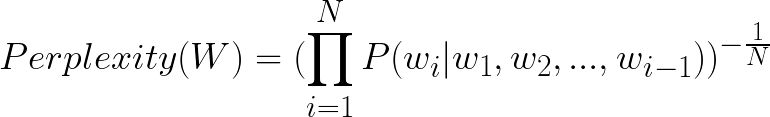
\includegraphics[width=0.8\textwidth]{statics/Furitsch/prod_var.png}
\end{center}
Es werden also die Wahrscheinlichkeiten aller Präfix/Suffix Kombinationen des Testsatzes in ein Produkt umgewandelt und dieses wird durch den negativen Durchschnitt poteziert.
Doch diese Variante bringt einige Probleme mit sich. Zum einen können ohne die Verwendung von Smoothing Techniken Nullwahrscheinlichkeiten mit in das Produkt einfließen was das Peodukt in jedem Fall 0 macht. Außerdem ist diese Variante unstabil bei sehr vielen sehr kleinen Werten da der Endwert dadurch immer kleiner wird.
Deshalb gibt es eine äquivalente Umformung
\begin{center}
	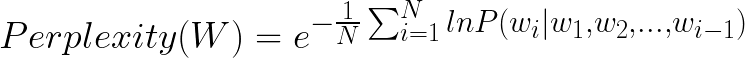
\includegraphics[width=0.8\textwidth]{statics/Furitsch/log_var.png}
\end{center}
Es werden alle ermittelten Wahrscheinlichkeiten logarithmiert, anschließend summiert, durch den negativen Wert der Anzahl der Wahrscheinlichkeitselementmenge geteilt. Dieser Wert wird in e-Funktion gegeben um anschließend einen endgültigen Wert zu bringen. Je niedriger dieser ist, umso besser konnte der Testsatz von dem Modell verhergesagt werden.\\ Das Logarithmieren dient dazu, vor allem sehr kleine Zahlen wieder größer zu skalieren, um mit ihnen besser arbeiten zu können. Da das Logarithmieren eine monotone Transformation ist, das bedeutet der Wert wird zwar verändert aber sein Verhältnis zu den anderen Werten wird nicht verändert. Durch die Logarithmusgesetzte wissen wir dass wir das Produkt nun in Summen umwandeln können und durch die E-Funtion machen wird das Logarithmieren wieder rückgängig und kehren zurück in den Raum der Wahrscheinlichkeit. Außerdem erlaubt sie uns auch den Exponenten der Produktform in einen Multiplikator umzuwandeln.
\begin{lstlisting}
def perplexity(model, test_data_tokens):
    grams = getGrams(len(test_data_tokens), test_data_tokens)
    accumulator = 0.0

    for gram_list in grams:
        for gram in gram_list:
            prefix = tuple(gram[:-1])
            suffix = gram[-1]
            if len(prefix) > 0:
                if prefix in model and suffix in model[prefix]:
                    propabilitie = model[prefix][suffix]
                    accumulator += math.log(propabilitie)
                else:
                    accumulator += math.log(1e-10)

    perplexity_result = math.exp(accumulator / -len(test_data_tokens))
    print(f"Perplexity: {perplexity_result}")
\end{lstlisting}
\subsection{Zukunft von N-Gramm Modellen}
\subsubsection{Vergleich zu Transformermodellen}
\quad Während n-Gram Modelle eine sehr effiziente und recht triviale Lösung für einfache Worterkennung sind ist es den modernen Modellen in einigen Punkten unterlegen. Zu erwähnen sind insbesondere die Transformer Modelle, welche insbesondere in der Lage sind, Kontexte von großen Texten viel besser modellieren können als n-Grame, da ihr Wahrscheinlichkeitsmodell nicht auf die Kontextlänge N-1 vorangegangenen Wörtern beschränkt ist. Außerdem haben sie damit eine erhöhte Flexibilität und gesteigerte Effizienz. Das sind dann keine einfachen Modelle mehr. Die Datenmenge, die benötigt wird, um solche Modelle zu trainieren ist noch viel größer als die von N-Gramen. Auch wenn bei einem N-Gram Modell schon zwei Wörter genügen würden werden sie dennoch erst mit großen Datenmengen nützlich. Dennoch lassen sich n-Gramme viel einfacher implementieren und sind deshalb für kleinere Projekte eine gute Wahl.
\subsection{Ausblick}
\quad Deshalb lässt sich auch sagen das vor allem im privaten Sektor und bei kleineren Projekten bei denen zum Beispiel kein langer Wortkontext wichtig ist n-Gramme weiterhin zum Einsatz kommen und auch weiterhin werden neue Ideen zur Verbesserung dieser Modelle kommen, welche das Modell relevant halten. Zum Beispiel bessere Glättungstechniken. Dennoch werden sich vor allem in State of the Art Projekte und große Firmen eher die Tranformermodelle etablieren da sie weitaus besser und effizienter sind. Erwähnenswert währen hierbei vor allem neuste Technologien wie ChatGPT4o.


% Bibliography
\clearpage
\begin{thebibliography}{9}

	\bibitem{AIML2024}
	AIML, \textit{Compare the different sequence models (RNN, LSTM, GRU, and Transformers)}, \url{https://aiml.com/compare-the-different-sequence-models-rnn-lstm-gru-and-transformers/}

	\bibitem{Spriesterbach2023}
	Kai Spriesterbach, \textit{Update: Geheimnis gelüftet! Soviele Parameter hat GPT-4}, \url{https://www.afaik.de/gpt-4-anzahl-parameter/}

	\bibitem{thamm}
	Alexander Thamm, \textit{Regelbasierte Systeme}, \url{https://www.alexanderthamm.com/de/data-science-glossar/regelbasiertes-system/}

	\bibitem{markert2019}
	Katja Markert, \textit{N-gram Modeling}, Institut für Computerlinguistik Uni Heidelberg

	\bibitem{scheffervanck2019}
	Tobias Scheffer und Thomas Vanck, \textit{Statistische Sprachmodelle}, Universtät Potsdam, \url{https://docplayer.org/115275693-Statistische-sprachmodelle.html} 2019. 

	\bibitem{jurafsky2023}
	Daniel Jurafsky and James H. Martin, \textit{Speech and Language Processing}, 3rd Edition, Pearson, 2023.

	\bibitem{dremio2023}
	Dremio, ``Data Sparsity,'' \url{https://www.dremio.com/wiki/data-sparsity/}, Accessed: June 1, 2024.

	\bibitem{foster2020}
	David Foster, \textit{Generative Deep Learning: Teaching Machines to Paint, Write, Compose, and Play}, O'Reilly Media, 2020.

	\bibitem{maucher2022}
	Prof. Dr. Johannes Maucher \url{https://griesshaber.pages.mi.hdm-stuttgart.de/nlp/04ngram/01ngram.html}, Accessed: June 1, 2024.

	\bibitem{gale1995}
	William A. Gale, "Good–Turing smoothing without tears," \textit{Journal of Quantitative Linguistics}, 1995.

	\bibitem{roshmita2023}
	Roshmita Dey , Accessed: June 1,\textit{Understanding Language Modeling: From N-grams to Transformer-based Neural Models} 2024.

	\bibitem{clarkGiorgoloLappin}
	Alexander Clark, Gianluca Giorgolo, and Shalom Lappin, \textit{Statistical Representation of Grammaticality Judgements: the Limits of
		N-Gram Models}, Department of Philosophy, King’s College London

	\bibitem{babukumar2010}
	A. Suresh Babu, Kumar P.N.V.S.Pavan
	\textit{Comparing Neural Network Approach with N-Gram Approach for Text Categorization},     January 2010International Journal on Computer Science and Engineering 2(1)

\end{thebibliography}

\end{document}
